\documentclass{article}

\renewcommand{\familydefault}{\sfdefault}  %serifenlose Schrift
\usepackage{helvet} % Schrift: Helvetica


\usepackage{graphicx,graphics,tikz}
\usepackage{amsmath}
\usepackage{amsthm}
\usepackage{amsfonts}
\usepackage{amssymb}
\usepackage{marvosym} % to be able to show male and female symbols with: \Female and \Male
\usepackage{gensymb}
\usepackage[graphics,tightpage,active]{preview}
\PreviewEnvironment{tikzpicture}
\newlength\imagewidth
\newlength\imagescale

\begin{document}

%\pgfmathsetlength{\imagewidth}{10cm} % desired displayed width of image
%\pgfmathsetlength{\imagescale}{\imagewidth/2000} % pixel width of image
% adjust scale of tikzpicture (and direction of y) such that pixel
% coordinates can be used for drawing overlays:
\usetikzlibrary{backgrounds}

\begin{tikzpicture}%[x=\imagescale,y=-\imagescale]


\begin{scope}[yshift=-0.35cm]
  \node [black,text centered, text width=5cm] at (-7,9.8) {Present-day conditions};
\node [black] at (-1.6,9.6) {Georeferenced Occurrences};


\begin{scope}[xshift=-11,yshift=8.1cm]
\node[draw=white, ultra thick,inner sep=0pt,outer sep=0pt] at (-7,0)
  {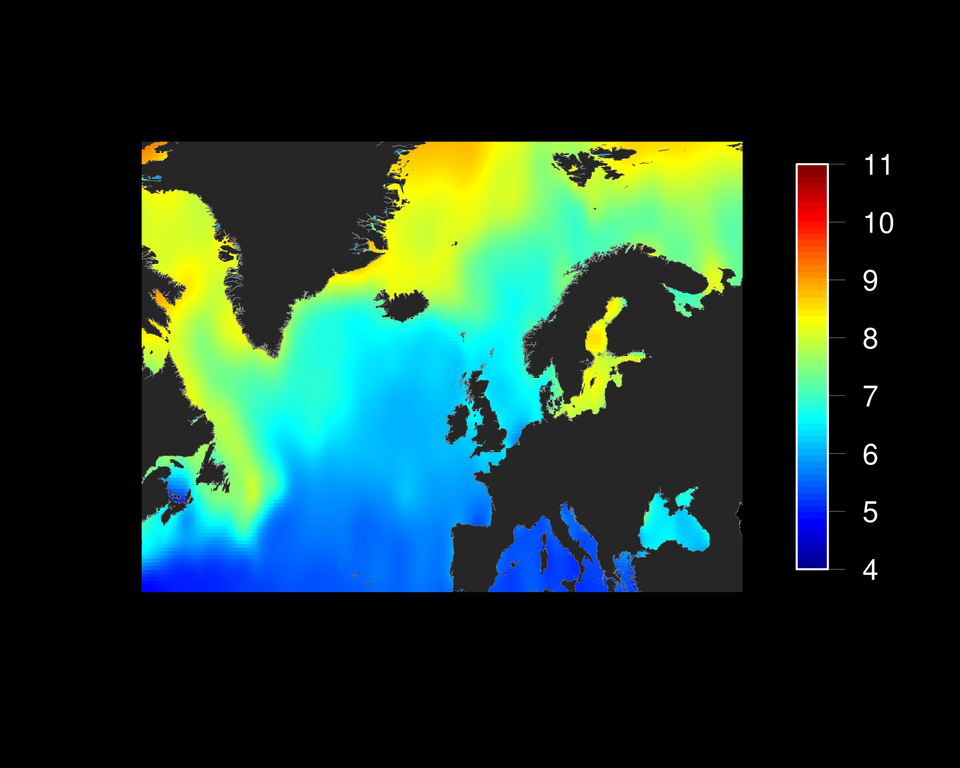
\includegraphics[width=2.5cm, bb=85 130 935 730, clip]{2011-12-18-dissox_2000.png}};
\node [white,scale=0.65] at (-7,0.7) {DA ($m^{-1}$)};
\end{scope}

\begin{scope}[xshift=-11*2,yshift=7.7cm]
\node[draw=white, ultra thick,inner sep=0pt,outer sep=0pt] at (-7,0)
  {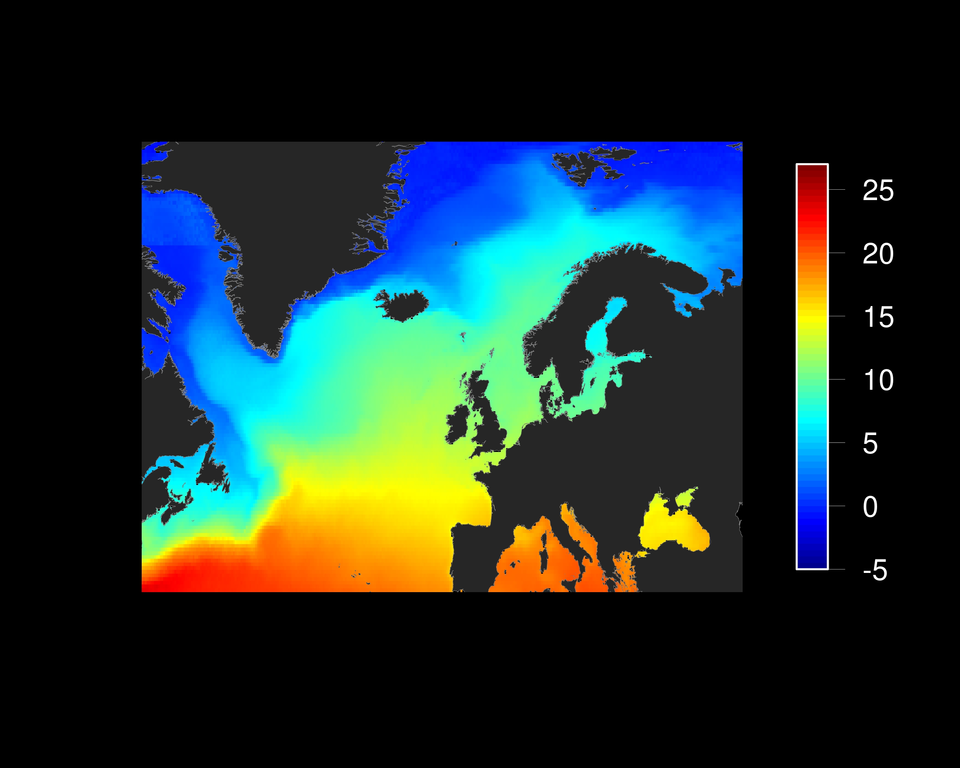
\includegraphics[width=2.5cm, bb=85 130 935 730, clip]{2011-12-18-sstmean_2000.png}};
\node [white,scale=0.65] at (-7,0.7) {SST (\textit{\celsius})};
\end{scope}


\begin{scope}[xshift=-11*3,yshift=7.3cm]
\node (conditions) [draw=white, ultra thick,inner sep=0pt,outer sep=0pt] at (-7,0)
  {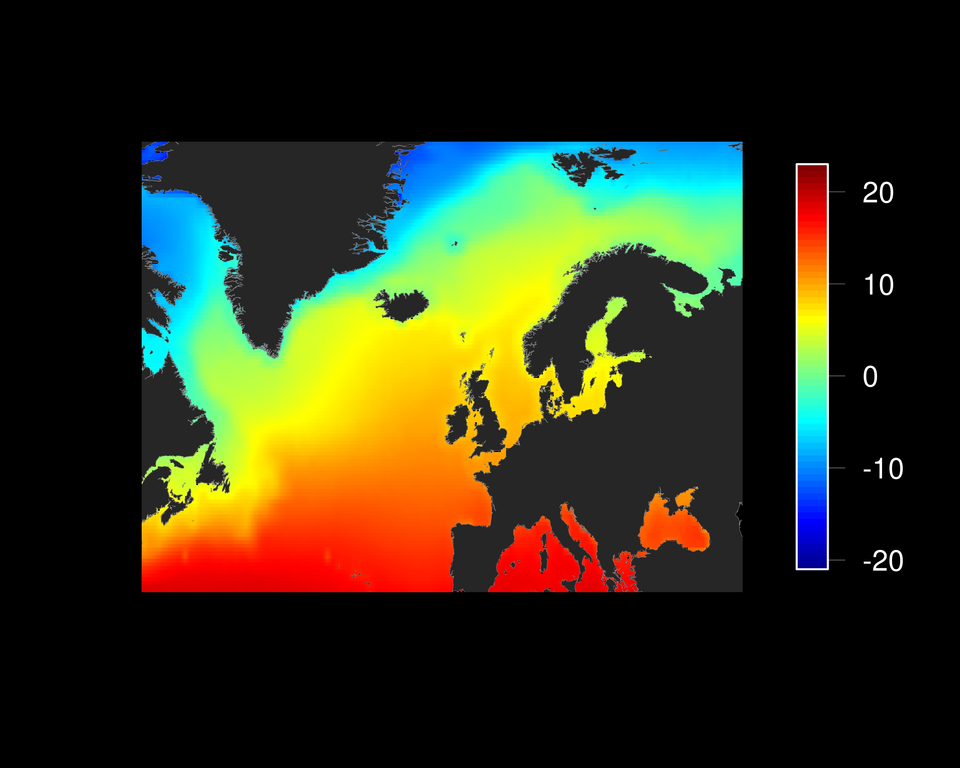
\includegraphics[width=2.5cm, bb=85 130 935 730, clip]{2011-12-18-satmean_2000.png}};
\node [white,scale=0.65] at (-7,0.7) {SAT (\textit{\celsius})};
\end{scope}

\begin{scope}[xshift=-11*4,yshift=7.7cm,xshift=7cm]
\node (occurrences) [draw=white, ultra thick,inner sep=0pt,outer sep=0pt] at (-7,0)
  {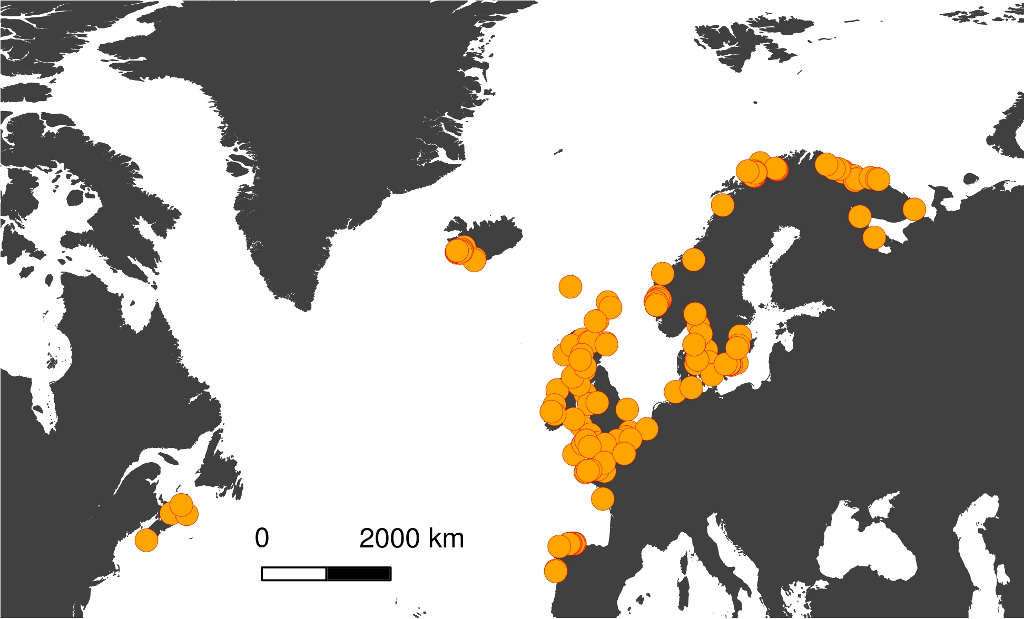
\includegraphics[width=4cm]{2011-12-18-Occurrences.png}};
\end{scope}

\end{scope}

\begin{scope}[shorten <=0.25cm]
\node (model) at (-5cm,5cm){};
\draw [->, line width=0.03cm] (occurrences) to [out=270,in=90] (model);>
\draw [->, line width=0.03cm] (conditions) to [out=270,in=90] (model);
\end{scope}

\node [text width=10cm,text centered] at (-5cm,4.9cm){Ecological Niche Model};

\begin{scope}[yshift=-4.5cm]
\node(2000point) at (-8.5cm,6.8cm) {2000};
\node(2100) at (-5cm,6.8cm) {2100 ?};
\node(2200) at (-1.5cm,6.8cm) {2200 ?};

\node (2000) [draw=white, ultra thick,inner sep=0pt,outer sep=0pt] at (-8.5cm,8.1cm)
  {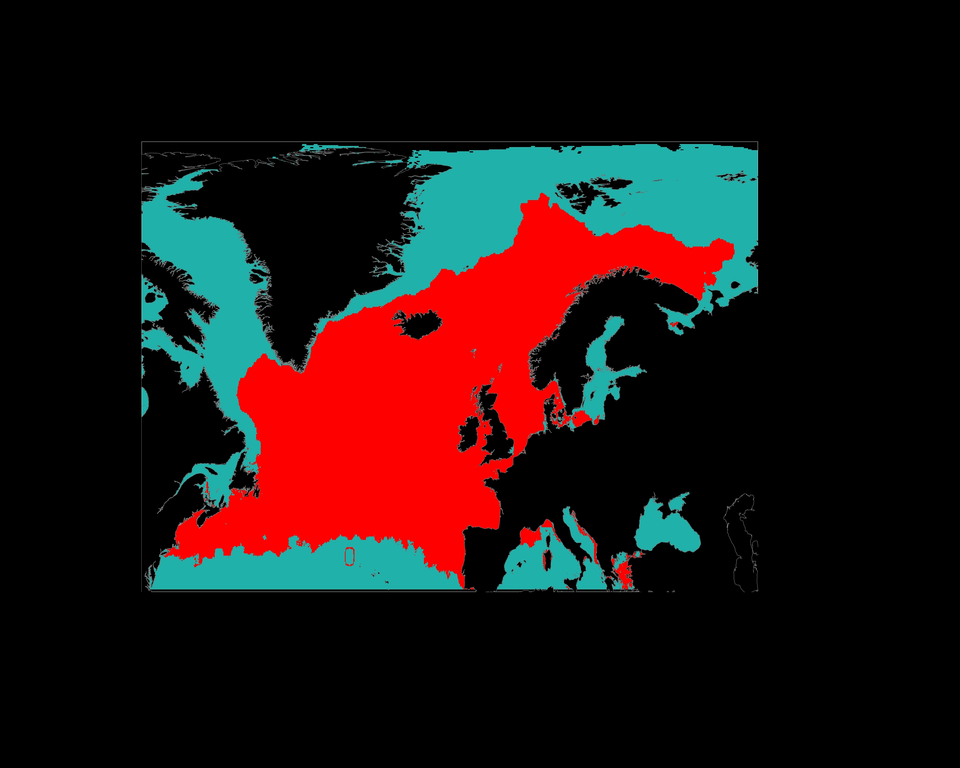
\includegraphics[width=2.5cm, bb=85 130 815 670, clip]{2011-12-18-Projection_binary_Present.png}};

\end{scope}

\begin{scope}[xshift=0cm,yshift=0.5cm]
\node[draw=white, ultra thick,inner sep=0pt,outer sep=0pt] at (-4.7cm,3.25cm)
  {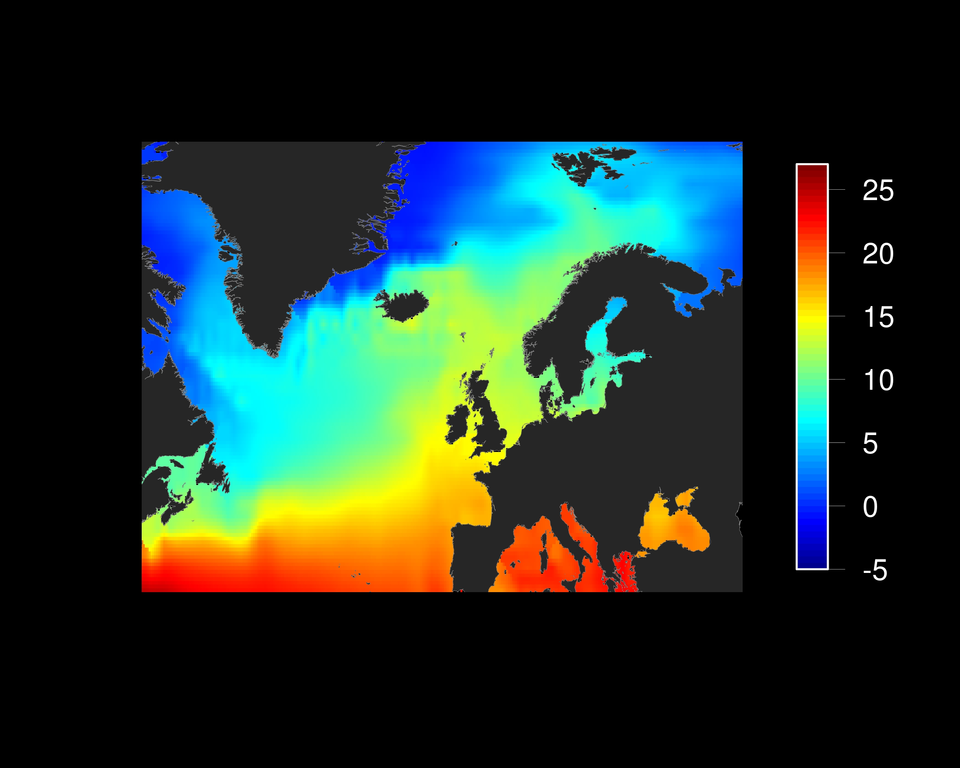
\includegraphics[width=2.5cm, bb=85 130 935 730, clip]{2011-12-18-sstmean_2100_A1B.png}};


\begin{scope}[xshift=-11,yshift=-10]
\node (conditions) [draw=white, ultra thick,inner sep=0pt,outer sep=0pt] at (-4.7cm,3.25cm)
  {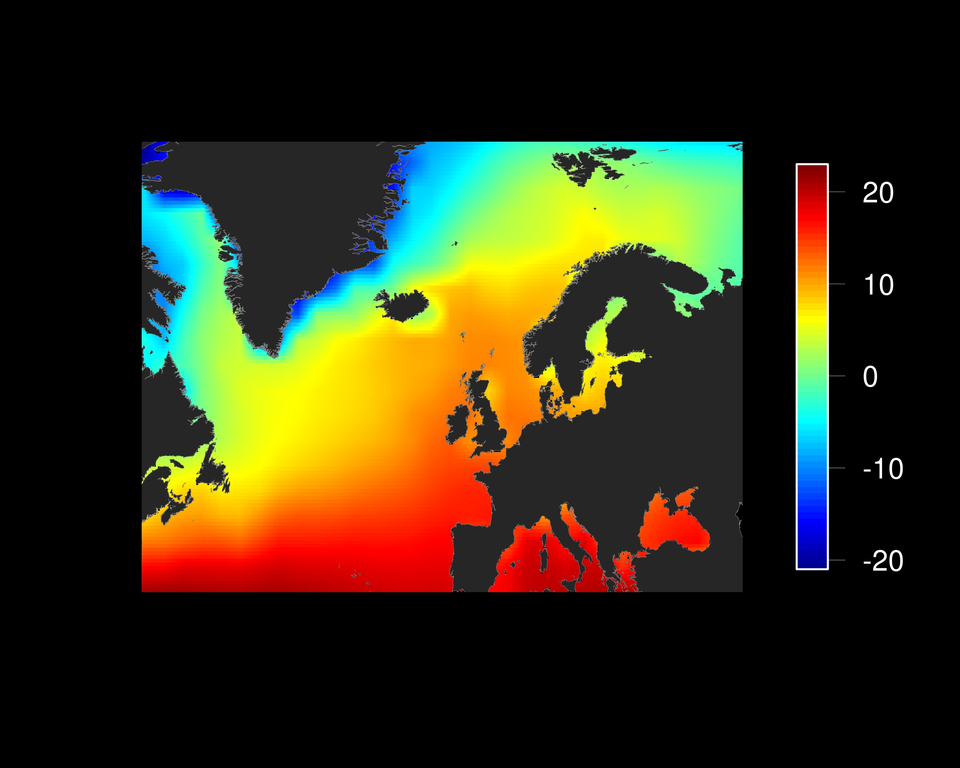
\includegraphics[width=2.5cm, bb=85 130 935 730, clip]{2011-12-18-satmean_2100_A1B.png}};
\node [white,scale=0.65] at (-4.2cm,4.3cm) {SST (\textit{\celsius})};
\node [white,scale=0.65] at (-4.7cm,3.95cm) {SAT (\textit{\celsius})};
\end{scope}
\end{scope}

\begin{scope}[xshift=3.5cm,yshift=0.5cm]
\node[draw=white, ultra thick,inner sep=0pt,outer sep=0pt] at (-4.7cm,3.25cm)
  {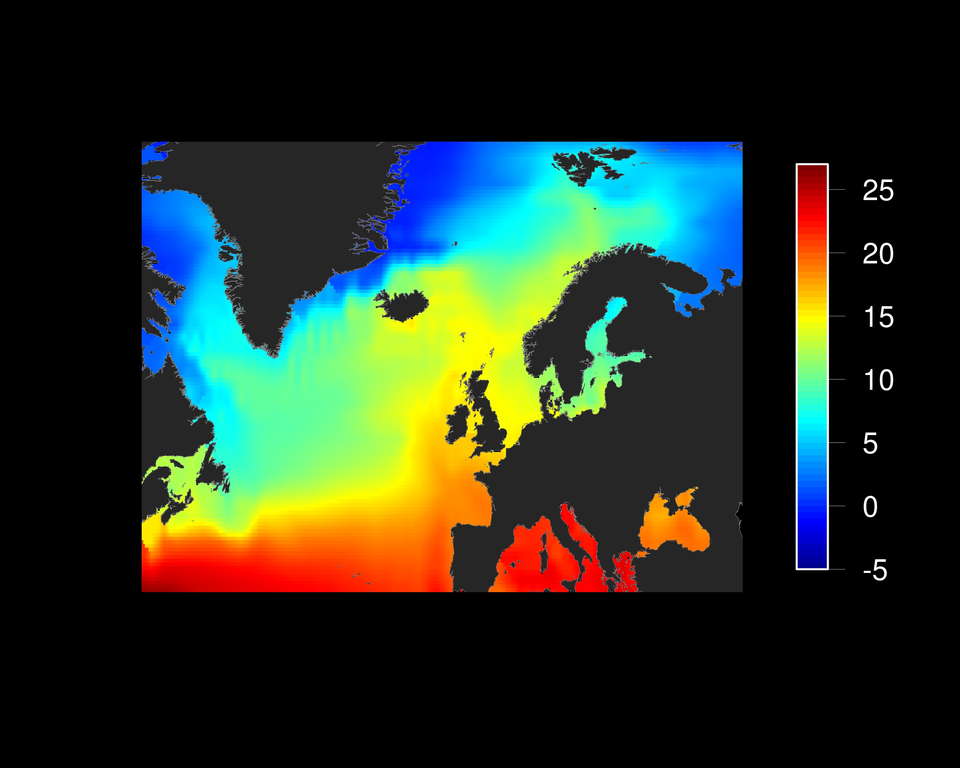
\includegraphics[width=2.5cm, bb=85 130 935 730, clip]{2011-12-18-sstmean_2200_A1B.png}};


\begin{scope}[xshift=-11,yshift=-10]
\node (conditions) [draw=white, ultra thick,inner sep=0pt,outer sep=0pt] at (-4.7cm,3.25cm)
  {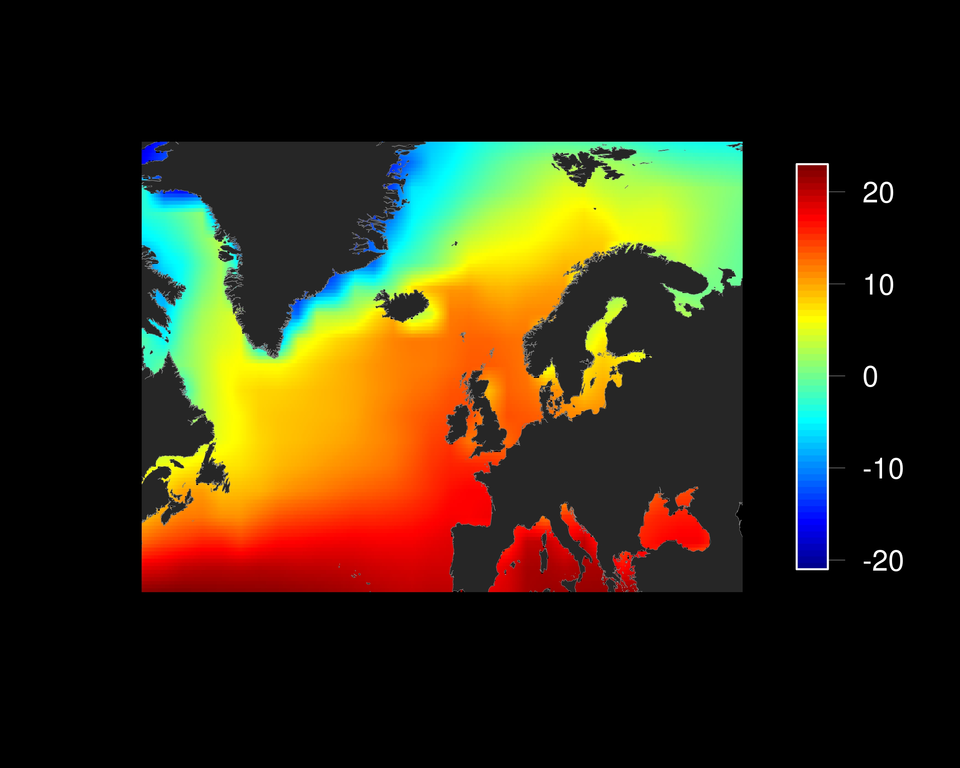
\includegraphics[width=2.5cm, bb=85 130 935 730, clip]{2011-12-18-satmean_2200_A1B.png}};
\node [white,scale=0.65] at (-4.2cm,4.3cm) {SST (\textit{\celsius})};
\node [white,scale=0.65] at (-4.7cm,3.95cm) {SAT (\textit{\celsius})};
\end{scope}
\end{scope}




\end{tikzpicture}

\end{document}